\documentclass{beamer}

%\mode<presentation>

\usetheme{Dresden}
\usecolortheme{beaver}
\setbeamercovered{transparent}

\usepackage[english]{babel}
\usepackage[latin1]{inputenc}
\usepackage{times}
\usepackage[T1]{fontenc} 
% Or whatever. Note that the encoding and the font should match. If T1
% does not look nice, try deleting the line with the fontenc.
\usepackage{amsmath}

\newcommand{\linespace}{\vskip 0.25cm}

%\definecolor{MyForestGreen}{rgb}{0,0.7,0} 
%\newcommand{\tableemph}[1]{{#1}}
%\newcommand{\tablewin}[1]{\tableemph{#1}}
%\newcommand{\tablemid}[1]{\tableemph{#1}}
%\newcommand{\tablelose}[1]{\tableemph{#1}}

%\definecolor{MyLightGray}{rgb}{0.6,0.6,0.6}
%\newcommand{\tabletie}[1]{\color{MyLightGray} {#1}}

% The text in square brackets is the short version of your title and will be used in the
% header/footer depending on your theme.
\title{Monte Carlo Search Tree and Its Applications}

% Sub-titles are optional - uncomment and edit the next line if you want one.
% \subtitle{Why does sub-tree crossover work?} 

% The text in square brackets is the short version of your name(s) and will be used in the
% header/footer depending on your theme.
\author[Magnuson]{Max Magnuson}

% The text in square brackets is the short version of your institution and will be used in the
% header/footer depending on your theme.
\institute[U of Minn, Morris]
{
  Division of Science and Mathematics \\
  University of Minnesota, Morris \\
  Morris, Minnesota, USA
}

% The text in square brackets is the short version of the date if you need that.
\date{April 25, 2015}

% Delete this, if you do not want the table of contents to pop up at
% the beginning of each subsection:
\AtBeginSection[]
{
  \begin{frame}<beamer>
    \frametitle{Outline}
    \tableofcontents
  \end{frame}
}

\begin{document}

\begin{frame}
  \titlepage
\end{frame}

% For a 20-25 minute senior seminar talk you probably want something like:
% - Two or three major sections (other than the summary).
% - At *most* three subsections per section.
% - Talk about 30s to 2min per frame. So there should probably be between
%   15 and 30 frames, all told.

\section{Introduction}

\begin{frame}
\frametitle{Monte Carlo Tree Search(MCTS)}
%cite british Go organisation http://www.britgo.org/learners/chessgo.html
\begin{itemize}
	\item AI algorithm
	\item Populates tree by randomly sampling simulations
	\item Probabilistic not deterministic
	\item Useful for problems with large search spaces
	\begin{itemize}
		\item Possible games of Chess: 10\textsuperscript{120}
		\item Game board for Chess: 8x8
		\item Possible games of Go: 10\textsuperscript{761}
		\item Game board for Go: 19x19
	\end{itemize}
\end{itemize}
\end{frame}

\section{Background}

\begin{frame}
\frametitle{Tree Structure}
What the nodes encode
\begin{itemize}
	\item intermediate state of the game
	\item estimated strategic value
	\item source node is the current game state
\end{itemize}
Edges in the tree represent actions
\end{frame}

\begin{frame}
\frametitle{TicTacToe Example}
\begin{figure}[h]
	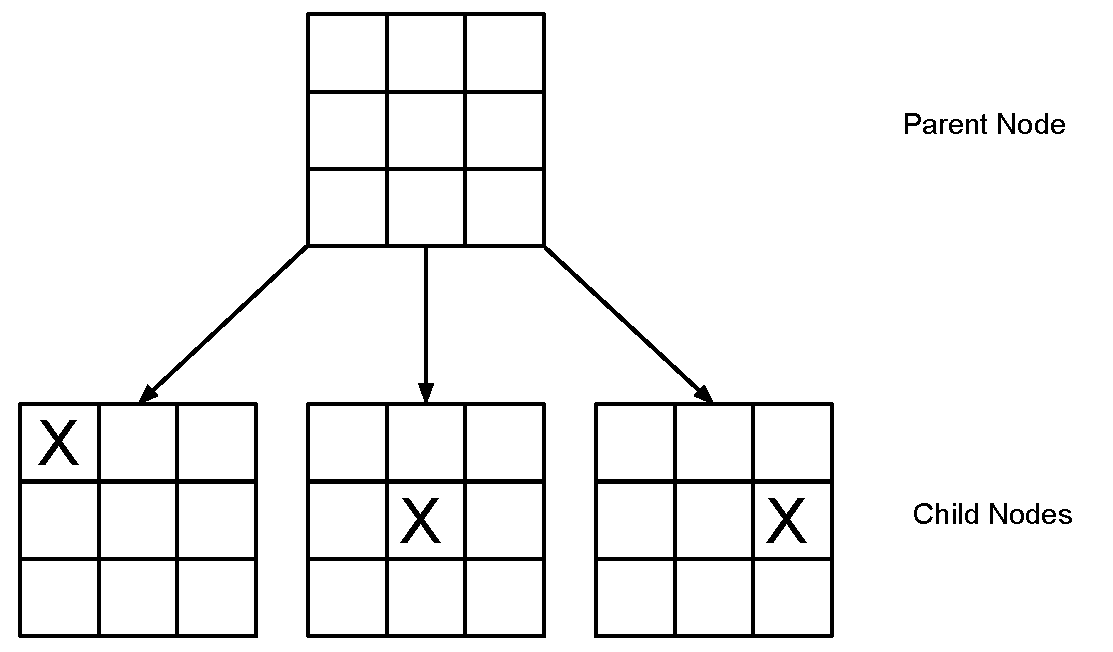
\includegraphics[width=8.5cm]{Diagrams/TicTacToeTree.pdf}
	\centering
\end{figure}
\end{frame}

\section{Applying MCTS to Go}

\section{Applying MCTS to Narrative Generation}

\section{Conclusion} 

\end{document}


